% ----------------------------------------------------------------------------
%
% ----------------------------------------------------------------------------

\documentclass[12pt, parskip=half]{scrartcl}       % KOMA-Skript für Artikel
\usepackage{setspace}

%% Präambel
\usepackage[english, ngerman]{babel} % deutsche typogr. Regeln + Trenntabelle
\usepackage[T1]{fontenc}             % interner TeX-Font-Codierung
\usepackage{lmodern}                 % Font Latin Modern
\usepackage[utf8]{inputenc}          % Font-Codierung der Eingabedatei
\usepackage[babel]{csquotes}         % Anführungszeichen
\usepackage{graphicx}                % Graphiken
\usepackage{booktabs}                % Tabellen schöner
\usepackage{amsmath}      % Mathematik
\usepackage{amssymb}      % Mathematische Symbole
\usepackage{float}
\usepackage{wrapfig}
\usepackage[pdftex]{hyperref}
\usepackage{subcaption}
\usepackage{url}
\hypersetup{
  bookmarksopen=true,
  bookmarksopenlevel=3,
  colorlinks,
  citecolor=blue,
  linkcolor=blue
}
\usepackage{scrhack} % unterdrückt Fehlermeldung von listings
\usepackage[backend=bibtex]{biblatex}
\addbibresource{/home/niklas/Documents/bibfile/bibliographie.bib}
\addbibresource{src/sources.bib}

%% Nummerierungstiefen
\setcounter{tocdepth}{3}     % 3 Stufen im Inhaltsverzeichnis
\setcounter{secnumdepth}{3}  % 3 Stufen in Abschnittnummerierung

\usepackage[nolist]{acronym}

\newcommand\litem[1]{\item{\bfseries#1.\space}}

\newcommand*{\N}{\mathbb{N}}
\newcommand*{\Z}{\mathbb{Z}}
\newcommand*{\Q}{\mathbb{Q}}
\newcommand*{\R}{\mathbb{R}}

% Code packages
\usepackage{listingsutf8} % Code mit UTF-8 Support
\usepackage{color,xcolor} % Farben definierbar als HTML, RGB, ...
\usepackage{textcomp}

\definecolor{alabasterGray}{HTML}{F7F7F7}
\definecolor{alabasterBlue}{HTML}{325CC0}
\definecolor{alabasterGreen}{HTML}{448C27}
\definecolor{alabasterPink}{HTML}{7A3E9D}
\definecolor{alabasterRed}{HTML}{AA3731}

\lstset{
  basewidth={0.5em,0.45em},
  extendedchars=true,
  backgroundcolor=\color{alabasterGray}, % background color (color or xcolor needed)
  basicstyle=\small\ttfamily,
  keywordstyle=\color{alabasterBlue},
  commentstyle=\color{alabasterRed},
  rulecolor=\color{black},          % frame color may change if not set (frame on comment, is comment-colored)
  stringstyle=\color{alabasterGreen},
  numberstyle=\tiny\color{gray},    %
  numbers=none,                     % where to put the line-numbers (none, left, right)
  numbersep=7pt,                    % margin between numbers and code
  stepnumber=1,                     % every n-th row will be numbered
  captionpos=b,                     % sets the caption-position to bottom
  frame=single,                     % adds a frame around the code
  keepspaces=true,                  % keeps spaces in text
  showtabs=false,                   % show tabs as special char
  showspaces=false,                 % show spaces as special char
  showstringspaces=false,           % show spaces in strings only as special char
  tabsize=2,                        % tabsize is 2 spaces
  breakatwhitespace=false,          % sets if automatic breaks should only happen at whitespace
  breaklines=true,                  % sets automatic line breaking
}
\lstset{
  literate={ö}{{\"o}}1
           {ä}{{\"a}}1
           {ü}{{\"u}}1
           % https://tex.stackexchange.com/questions/17739/listings-package-how-to-highlight-math-operators
           {true}{{{\color{alabasterPink}true}}}4
           {false}{{{\color{alabasterPink}false}}}5
           {TRUE}{{{\color{alabasterPink}TRUE}}}4
           {FALSE}{{{\color{alabasterPink}FALSE}}}5
           {True}{{{\color{alabasterPink}True}}}4
           {False}{{{\color{alabasterPink}False}}}5
}
\expandafter\def\expandafter\UrlBreaks\expandafter{\UrlBreaks\do\-\do\\/}

\begin{document}

\titlehead{
\includegraphics[width=\textwidth]{src/Logo_THM_CG_FB06.png}}

%% Titelseite
\subject{Manusskript}
\title{Progressive Web Apps}
\subtitle{Kurs \enquote{Hauptseminar -- Mobile Techonologies}}
\author{Niklas Deworetzki}
\date{\today}
\maketitle

\spacing{1.16} % Spacing entspricht Arial 12 - Zeilenabstand 1.3

\vspace*{1.5cm}
\section*{\centerline{Zusammenfassung}}

Diese Arbeit befasst sich mit Progressive Web Applications.




\newpage

\tableofcontents
\newpage

\section{Einleitung}

% TODO Einleitung
https://medium.com/@amberleyjohanna/seriously-though-what-is-a-progressive-web-app-56130600a093

\acp{pwa} werden immer relevanter.
Ergänzendes Element zwischen herkömmlicher Anwendung und Website.
Was kann man damit machen? Worum geht's eigentlich?

\section{Was ist eine \ac{pwa}?}

Der Begriff \acl{pwa} beschreibt eine Kategorie von Webanwendungen, welche eine Reihe an Eigenschaften erfüllen, um das Erlebnis einer nativen Anwendung in modernen Browsern zu bieten.
Geprägt wurde dieser Begriff von Alex Russell, welcher in seinem Blog\cite{russell_pwaescapingtabs} beschreibt, wie durch die Weiterentwicklung und Standardisierung von Browsern und Webtechnologien eine neue Art von Anwendung entstanden ist.
Diese Kategorie von Anwendungen entspreche dem nächsten Schritt in einer Reihe von Technologien, die versuchen, Entwicklern die Möglichkeit zu geben, mit nur einer plattformübergreifenden Anwendung auf plattformspezifische Ressourcen zuzugreifen.

Diese Kategorie von Webanwendungen ist also eine Art Nachfolger auf Technologien wie \enquote{Universal Windows Platform}-Apps\cite{msdocs_uwp} von Microsoft oder die von W3C standardisierten \enquote{Packaged Web Apps}\cite{w3c_packagedwebapps}, welche auch als \enquote{Widget} bekannt sind.
Der Begriff \enquote{Progressive} in \acl{pwa} steht für \enquote{Progressive Enhancement} (fortschreitende Verbesserung) und beschreibt ebendiese Vorgehensweise, eine Webanwendung auf möglichst vielen Geräten mit verschiedenen Kapazitäten nutzbar zu machen.
Die Idee dabei ist es, eine Grundversion der Anwendung zu erstellen, die auf jedem Gerät funktionieren kann.
Weitere Funktionalität für potentere Geräte werden dann auf diese Grundversion aufgebaut.

Da der Begriff der \ac{pwa} zusammen mit den notwendigen Technologien über einen längeren Zeitraum gewachsen ist, gibt es keine feste Definition für das, was eine \ac{pwa} ausmacht.
Die Beschreibung einer \ac{pwa} basiert vielmehr auf einer Menge an Eigenschaften, die eine Anwendung innehaben kann.
Im Folgenden werden daher einige Eigenschaften zusammengetragen und erläutert, die immer wieder für die Beschreibung von \acp{pwa} verwendet werden.
Ein besonderer Schwerpunkt wird dabei auf die Standpunkte der Google- und Mozilla-Entwickler gelegt, da diese treibende Kraft beim Entwickeln von \acp{pwa} sind und gemeinsam die Fähigkeiten dieser Gruppe von Anwendungen ausbauen.

\newpage % TODO: Eine Seite mehr an dieser Stelle. Nachher vielleicht anpassen?

Die gesammelten Eigenschaften einer \ac{pwa} lassen sich dabei in folgende Kategorien einteilen, in welcher sie auch erläutert werden.

\begin{enumerate}
  \litem{Grundlegende Eigenschaften} Eigenschaften einer \ac{pwa}, die dem Charakter einer \ac{pwa} entsprechen und ohne die ein Funktionieren der Anwendung nicht möglich wäre.

  \litem{Verbreitete Eigenschaften} Eigenschaften einer \ac{pwa}, welche von verschiedenen Quellen genannt werden, aber nicht unbedingt notwendig für das Funktionieren der Anwendung sind.

  \litem{Designmerkmale} Eigenschaften einer \ac{pwa}, die sich positiv auf das Nutzererlebnis auswirken.
\end{enumerate}


\subsection{Grundlegende Eigenschaften}

Die wohl wichtigste Eigenschaft einer \ac{pwa} ist, dass sie installierbar sein muss.
Wenn ein Nutzer eine Website besucht, welche als \ac{pwa} agiert, so kann dem Nutzer eine Installationsaufforderung gezeigt werden.
Durch den Installationsvorgang werden teile der Anwendung auf dem lokalen Gerät gespeichert und die \ac{pwa} optisch zu den nativen Anwendung integriert.
Ob diese Integration nun über das Hinzufügen eines Desktopicons, eine Verknüpfung auf dem Startbildschirm oder auch nur über einen Eintrag in einem Anwendungslauncher erfolgt, ist dabei vom unterliegenden System abhängig.
Auf einem Android-Gerät wird es beispielsweise sinnvoll sein, die \ac{pwa} als Icon auf dem Startbildschirm anzuzeigen.
Auf einem Windows-Gerät stattdessen wird dem Nutzer eine Verknüpfung auf dem Desktop lieber sein.
Da die \ac{pwa} nicht eigenständig entscheiden kann, welches Gerät der Nutzer verwendet und wohl unmöglich die Fähigkeit besitzt, für jedes Gerät die entsprechende Konfiguration durchzuführen, muss der Installationsvorgang durch den Browser unterstützt und verwaltet werden.

Beim anschließenden Ausführen einer installierten \ac{pwa} ist erneut Unterstützung vom Browser notwendig.
\acp{pwa} als Webanwendung werden mit Webtechnologien wie HTML und CSS aufgebaut und erhalten ihre Funktionalität durch JavaScript.
Betriebsysteme bieten jedoch nur eine begrenzte Unterstützung für Programmformate, die nativ ausgeführt werden können.
Abgesehen von Skriptdateien wie etwa Shell-Scripts für Linux oder Command-Files für Windows, die in einem betriebsystemabhängigen Format geschrieben sein müssen, wird meist nur die Ausführung von Binärformaten unterstützt\cite{fisher_executablelist}.
Es wird also Hilfe vom Browser benötigt, welcher die installierte \ac{pwa} verwaltet und daher alle benötigten Dateien laden und ausführen kann.
Zudem ist es dem Browser möglich, für die Ausführung einer \ac{pwa} bestimmte Regeln festzulegen.
In Google Chrome beispielsweise wird jede \ac{pwa} in einem eigenen Fenster gestartet, wodurch das Nutzererlebnis einer nativen Anwendung entstehen soll\cite{googledevs_pwa}.


Durch den Installationsprozess werden nur Teile \ac{pwa} lokal auf dem Gerät gespeichert.
Der Grund dafür ist, dass es meist nicht genügt, eine Website einfach vollständig zu kopieren, um sie offline verfügbar zu machen.
Viele Webanwendungen, wie beispielsweise die \ac{pwa} von Twitter\cite{twitter_pwa}, basieren darauf stetig neue Inhalte von einem Server abzufragen.
Die Verwaltung, welche Inhalte offline verfügbar sein sollen und welche nicht, geschieht über sogenannte \enquote{Service Worker}.
Dadurch dass jede \ac{pwa} lokale und entfernte Inhalte verwalten muss, ist das vorhandensein von Service Workern, eine weitere Eigenschaft, die jede \ac{pwa} besitzt.

Eine Voraussetzung der Service Worker erzwingt eine weitere Eigenschaft aller \acp{pwa}.
Service Worker können laut Spezifikation nur auf Seiten ausgeführt werden, die über HTTPS ausgeliefert werden.
Der Grund dafür ist, dass Service Worker die Fähigkeit besitzen, Anfragen zu filtern, umzuleiten und auszulesen.
Die verschlüsselte Verbindung bei HTTPS verhindert dabei die Manipulation durch Dritte beim Ausliefern des Service Worker.
So soll sichergestellt werden, dass Service Worker nicht für das Ausspionieren von Daten genutzt werden\cite{ServiceWorker_explained}.

% TODO: Bin unzufrieden mit dem Abschnitt.
Die letzte grundlegende Eigenschaft einer \ac{pwa} ergibt sich aus der Herkunft dieser.
Wie bei einer herkömmlichen Website geschieht die Auswahl der Inhalte, die angezeigt werden sollen, über eine URL.
Folglich sollte jeder Zustand der \ac{pwa} durch eine URL erzeugbar und erreichbar sein.
Dadurch ergeben sich viele Vorteile, vor allem in Hinsicht auf die Interaktion mit der \ac{pwa}.
Ist nämlich der angezeigte Inhalt allein von der URL abhängig, so genügt die URL, um Inhalte zu verbreiten und zu teilen.
Dadurch wird die Anwendung komplett unabhängig von Gerät oder Nutzer, was dem progressiven Design entspricht.
Auch die soziale Komponente dieses uneingeschränkten Teilens ist nicht zu unterschätzen.


\subsection{Häufige Eigenschaften}

Die im Folgenden genannten Eigenschaften, werden häufig bei \acp{pwa} angetroffen, sind jedoch nicht notwendig für die Funktionalitäten, die eine \ac{pwa} ausmachen.
Größtenteils entstehen diese Eigenschaften durch Marketing für \acp{pwa}.

Beispielsweise wird von den Google Entwicklern bei einer Erklärung zu \acp{pwa} mit der Aussage geworben, dass 53\% der Nutzer eine Website wieder verlassen, falls sie länger als drei Sekunden lädt.\cite{googledevs_performance}
Dies suggeriert, dass \acp{pwa} automatisch schnellere Ladezeiten besitzen.
% TODO: Erklären, warum es wirklich besser ist. (Analysesoftware bereitgestellt, Frameworks)
% Walton "Real World Performance"
% Bishop "Are PWA faster?"
% Faletski "Speed"

% TODO API Nutzung

\subsection{Designmerkmale}

Wie sehr \acp{pwa} an native Anwendungen angelehnt sind, lässt sich häufig in den Designmerkmalen der Anwendungen wiedererkennen.

Das bereits erwähnte Starten der Anwendung in einem eigenen Fenster beispielsweise soll dem Nutzer das Gefühl verleihen, eine native, installierte Anwendung zu starten.
Zusätzlich gibt es die Möglichkeit, ein Farbschema für die gesamte Anwendung festzulegen.
Der Effekt eines solchen Farbschemas ist, dass die Steuerungskomponenten des Browsers farblich an die \ac{pwa} angepasst werden können.
Dadurch wirkt die Anwendung für den Nutzer einheitlich und es wird versteckt, dass die \ac{pwa} eigentlich nur im Browser angezeigt wird und keine eigenständige Anwendung ist.
Es gibt das gleiche Prinzip bei nativen Anwendungen, die mit Farbschemen die Komponenten des Systems einfärben können, um die gesamte angezeigte Oberfläche einheitlich erscheinen zu lassen.

% TODO: Notifications und Einbindung in native Oberflächen.



\section{Technische Voraussetzungen}

%TODO Einleitung

\subsection{Installationsformat}

Das Installieren einer \ac{pwa} entspricht Größtenteils dem Setzen eines Lesezeichens bei einer herkömmlichen Website.
Dem Browser wird mitgeteilt, dass eine Referenz auf diese Website in eine lokale Sammlung aufgenommen werden soll.
Moderne Browser, wie Google Chrome oder Firefox, können Verknüpfungen für beliebige Websites auf dem Desktop oder im Startmenü erstellen.\cite{mozillasupport_desktopshortcut}\cite{businessinsider_desktopshortcut_chrome}
Dieses Verhalten entspricht genau dem, was bei einer \ac{pwa} gewünscht ist, welche auch zwischen den nativen Anwendungen auf dem Desktop oder Startbildschirm des Gerätes angezeigt werden sollen.

Bei der Installation einer \ac{pwa} wird lediglich auf diesen Fähigkeiten des Browsers aufgebaut.
Wie bei einer Verknüpfung für eine herkömmliche Website ist es auch bei einer \ac{pwa} gewünscht, ein Icon zusammen mit einem Namen anzuzeigen.
Es fehlen jedoch einige Eigenschaften bei einer solchen Verknüpfung, die eine native App besitzen würde.
Für die Konfiguration dieser Informationen existiert ein normiertes Format, welches mit einer \ac{pwa} ausgeliefert wird.
In dem sogenannten \textit{Manifest} einer Website werden die Eigenschaften über \ac{json} festgelegt.

Die Einbindung des Manifests geschieht im Header einer \ac{pwa}.
Dort kann über ein gewöhnliches \texttt{link}\-Tag eine Manifestdatei eingebunden werden.

\begin{figure}[h]
\begin{lstlisting}[language=HTML]
                <link rel="manifest" href="/manifest.json">
\end{lstlisting}
\caption{Einbindung einer Manifestdatei}
\label{fig:html_linkmanifest}
\end{figure}

Die Spezifikation der Eigenschaften in der Manifestdatei geschieht über Schlüssel\-Werte\-Paare.
Das Definieren der Schlüssel \enquote{short\_name}, \enquote{name}, \enquote{icons}, \enquote{start\_url} und \enquote{display} ist dabei verpflichtend.

\enquote{short\_name} und \enquote{icons} beschreiben das Aussehen der Verknüpfung.
Der Schlüssel \enquote{icons} ist im plural, da in der Manifestdatei mehrere Icons in verschiedenen Auflösungen angegeben werden sollten.
So kann je nach Auflösung des Gerätes das am besten passende Icon vom Browser gewählt werden.
Der lange Name \enquote{name} wird für Installationsdialoge und als Beschriftung der Verknüpfung verwendet.
Zusätzlich sollte der verkürzte Name angegeben werden, welcher alternativ angezeigt wird, wenn weniger Platz vorhanden ist.\cite{chromedevs_manifestname}
Dies kann bei mobilen Geräten der Fall sein.

Mit dem Schlüssel \enquote{display} wird gesteuert, wie der Browser die \ac{pwa} anzeigt.
Hier kann als Wert \enquote{fullscreen}, \enquote{standalone} oder \enquote{browser} angegeben werden.
Bei jedem dieser Werte wird die \ac{pwa} in einem eigenständigen Fenster ausgeführt.
Die Werte \enquote{fullscreen} oder \enquote{standalone} blenden dabei die Anzeigeelemente des Browsers aus.
Es wird also keine Navigationsleiste oder URL angezeigt.
Ist der Wert \enquote{fullscreen} gewählt, so wird die \ac{pwa} im Vollbildmodus gestartet, sodass zusätzlich die Anzeigeelemente des Betriebsystems ausgeblendet sind.
Durch den Wert \enquote{browser} werden die Anzeigeelemente des Browsers wie bei einer herkömmlichen Website angezeigt.\cite{googledev_manifest}

Der Wert \enquote{start\_url} ist wichtig für das Verhalten einer \ac{pwa}.
Da eine \ac{pwa} wie ein Lesezeichen an jeder Unterseite der Anwendung installiert werden kann, genügt es nicht, bloß die aktuelle URL abzuspeichern.
Wenn ein Nutzer beispielsweise gerade sein Profil betrachtet und sich an dieser Stelle entschließt, die \ac{pwa} zu installieren, so würde er bei erneutem Starten der \ac{pwa} immer wieder zu seinem Profil zurückkehren, wenn die Eigenschaften eines herkömmlichen Lesezeichens übernommen werden.
Es ist aber bei einer Anwendung meistens erwünscht, in ein zentrales Menü (Startmenü) herein zu starten, welches zu Beginn angezeigt wird.
Die URL für dieses Startmenü wird also an dieser Stelle angegeben.

Alle weiteren Schlüssel sind optional.
Sie dienen der Verbesserung des Nutzererlebnis, können aber auch weggelassen werden, wenn ein Einsatz nicht sinnvoll ist.

Der Schlüssel \enquote{description} gibt eine Beschreibung der \ac{pwa}.
Diese kann zusammen mit der Verknüpfung angezeigt werden.
Ein anderer optionaler Schlüssel ist \enquote{scope}, mit welchem die Reichweite der \ac{pwa} angegeben werden kann.
So kann eine \ac{pwa} als Teil in eine existierende Website integriert werden, indem nur eine bestimmte Gruppe an Routen zugewiesen wird.\cite{webdev_addmanifest}

Weitere optionale Schlüssel dienen der Integration in den Browser.
Über den Schlüssel \enquote{background\_color} lässt sich beispielsweise eine Farbe festlegen, die vom Browser beim Laden der Anwendung angezeigt wird, wenn noch keine Inhalte sichtbar sind.
So lässt sich ein Farbschema wie bei einer nativen Anwendung imitieren.
Der Schlüssel \enquote{theme\_color} passt zusätzlich noch die Farbe der Browserkomponenten an, sodass ein einheitliches Farbschema für die \ac{pwa} entsteht.



\subsection{Datenverwaltung durch Service Worker}

Wie bereits erwähnt, werden bei einer \ac{pwa} Inhalte sowohl von lokalen Quellen als auch über das Netzwerk geladen.
Da eine \ac{pwa} vor der Installation wie eine herkömmliche Website agiert, ist es nicht möglich, einfach im Quelltext der Anwendung die lokal installierten Inhalte anzugeben.
Diese sind vor der Installation gar nicht lokal verfügbar, wodurch das Abrufen dann zu einem Fehler führen würde.
Auch das Ausliefern von zwei Versionen an den Nutzer, die einmal für den \textit{Online Gebrauch} und einmal für den \textit{Offline Gebrauch} gedacht sind, ist nicht möglich, da die Installation durch den Browser durchgeführt wird, welcher die aktuell angezeigte Seite installiert.
Dadurch würde die Online-Version der Anwendung dauerhaft verwendet werden, was dem Sinn der Installation widerspricht.

\begin{wrapfigure}{r}{0.53\textwidth}
  \centering
  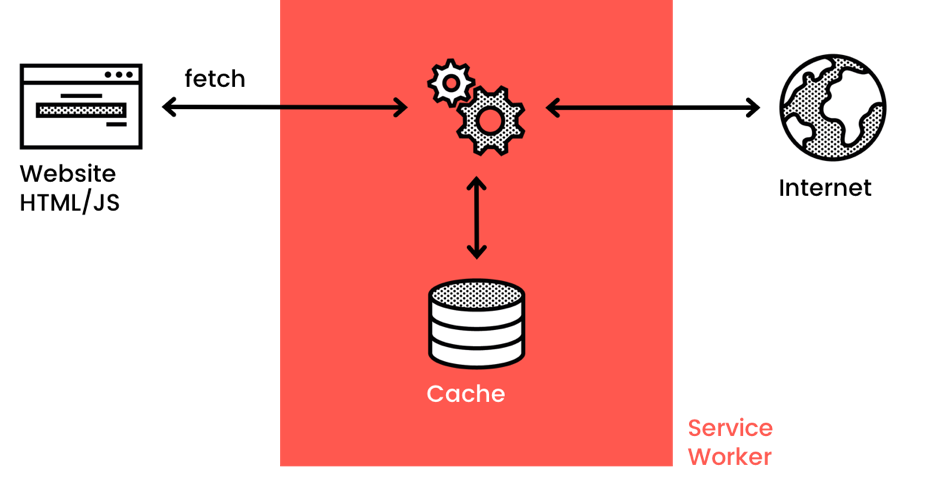
\includegraphics[width=1\linewidth]{src/ServiceWorker-Heise.png}
  \caption{Service Workers als Proxy\cite{src_serviceworker_heise}}
  \label{fig:heise_serviceworker}
\end{wrapfigure}

Folglich ist es also notwendig, einheitlich die Inhalte aus dem Netzwerk abzurufen, da sie dort immer erhältlich sind.
Werden diese Netzwerkanfragen dann noch lokal abgefangen, kann überprüft werden, ob ein Inhalt bereits lokal erhältlich ist.
Wenn dies der Fall ist, so ist es möglich, die Anfrage umzuleiten, sodass die lokalen Ressourcen verwendet werden.
Für die lokale Verwaltung von Inhalten sind die sogenannten \enquote{Service Worker} zuständig, dessen Funktionsweise im folgenden näher erläutert wird.

Wie andere Arten der \enquote{Worker} sind Service Worker auch ein JavaScript-Programm, das in einem eigenen Kontext läuft.
Dieser Kontext ermöglicht die Verwendung mehrerer Threads in JavaScript, da jeder Kontext in einem eigenen Thread laufen kann.
So ist ein Service Worker im Hintergrund aktiv und kann dort auf Events reagieren.
Dabei haben Service Worker jedoch keinen direkten Zugriff auf das \ac{dom} der \ac{pwa}.

In dem globalen Kontext der Service Worker befindet sich ein Cache-Objekt, welches den lokalen Speicher der \ac{pwa} repräsentiert.\cite{w3c_serviceworker_nightly}
Dieser Cache muss zunächst populiert werden, was entweder bei der Installation der \ac{pwa} oder zu späterem Zeitpunkt mit der ersten Anfrage einer Ressource geschehen kann.\cite{ServiceWorker_explained}
Anschließend kann bei Anfragen von gecachten Inhalten, auf den Cache verwiesen werden.

Das Reagieren auf Anfragen geschieht über ein \enquote{fetch}-Event, auf welches Service Worker reagieren können.
Für dieses Event kann eine Funktion registriert werden, welche ein Event-Objekt als Parameter akzeptiert.
Das Event-Objekt enthält alle Informationen über die angeforderte Ressource und kann manipuliert werden, um auszuwählen, von wo die Ressource geladen werden soll.
Wenn der Cache bereits populiert ist, ist die Auswahl über den Cache trivial.

\begin{figure}[h]
\begin{lstlisting}[language=java]
  self.addEventListener('fetch', function(event) {
    event.respondWith(caches.match(event.request)
      .then(cachedResponse => cachedResponse || fetch(event.request)))
  });
\end{lstlisting}
\caption{Auswahl von Ressourcen aus dem Cache.\cite{heise_pwa2}}
\label{fig:js_cache}
\end{figure}

Wie in Abbildung \ref{fig:js_cache} dargestellt, wird eine anonyme Funktion für das \enquote{fetch}-Event registriert.
Diese Funktion legt fest, dass auf die Anfrage des \enquote{fetch}-Event eine Antwort aus dem Cache gesucht werden soll.
Wenn die angeforderte Ressource im Cache vorhanden ist, wird sie als Ergebnis der Anfrage festgelegt.
Andernfalls wird eine Anfrage über das Netzwerk gesendet, um die Ressource abzurufen.

% TODO Gegenlesen: Ressource vs. Inhalt

Durch Service-Worker ist es also möglich, einen Cache in jede Website einzubinden.
Da diese im Hintergrund arbeiten und auf bereits vorhandene Technologien aufbauen, ist es nicht einmal nötig, eine bereits vorhandene Website anzupassen, um den Cache zu implementieren.

% TODO Einfügen: Nur über HTTPS weil Proxy

\subsection{Interaktion mit Nutzern}

Eine weiteres Merkmal von \acp{pwa}, welches herkömmliche Websites nicht besitzen, ist die Art und Weise, wie mit Nutzern interagiert wird.
Native Anwendungen können auf Ressourcen des Betriebsystems zugreifen, um mit dem Nutzer zu interagieren selbst wenn die Anwendung nicht aktiv vom Nutzer verwendet wird.
Weit verbreitet ist beispielsweise das Verwenden von Push-Notifications\cite{businessofapps_pushnotificationstatistics}, um Nachrichten oder Informationen an den Nutzer zu leiten.

\acp{pwa} sind ebenso in der Lage, Push-Notifications zu senden, was sie von herkömmlichen Websites abgrenzt.
Diese können auch Benachrichtigungen senden, jedoch nur, wenn der Nutzer aktiv eine Seite betrachtet.
Durch Service-Worker, welche unabhängig eines Seitenaufrufs ausgeführt werden, können \acp{pwa} auch Benachrichtigungen senden, ohne dass die \ac{pwa} geöffnet ist\cite{ejaz_progressive_pushnotifications}.

\begin{figure}[h]
  \centering
  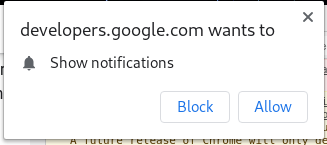
\includegraphics[width=0.4\linewidth]{src/permission-request-chrome.png}
  \caption{Google Chrome fragt um die Zustimmung des Nutzers.}
  \label{fig:chrome_permission}
\end{figure}

Zunächst muss ein Nutzer zustimmen, dass er Benachrichtigungen von einer Website oder \ac{pwa} erhalten will.
Falls die Zustimmung erteilt wird, wird dies für die entsprechende Website oder \ac{pwa} gespeichert, sodass eine Zustimmung nur ein einziges Mal eingeholt werden muss, so lange der Nutzer nicht im Nachhinein die Berechtigung widerruft.

Auf einer geöffneten Website genügt die Zustimmung des Nutzers, um eine Benachrichtigung anzuzeigen.
Der beim Seitenaufruf ausgeführte JavaScript-Code kann aktiv eine Benachrichtigung erstellen und anzeigen.
Eine \ac{pwa}, die nicht ausgeführt wird, kann auf diesen Weg keine Benachrichtigung anzeigen.
Auch der Service-Worker kann nicht aktiv eine Benachrichtigung erstellen, da dieser nur auf externe Events reagiert.

% TODO Wie läuft das Senden / Empfangen eines Events ab (w3c Push API, Atul Medium)

\subsection{Interaktion mit Hardware}

\subsection{Browserspezifische Voraussetzungen}


\section{Vorteile von PWAs}

\section{Kritik an PWAs}

\section{Fazit}

\newpage

\spacing{1}

\begin{acronym}
  \acro{pwa}[PWA]{Progressive Web App}
  \acro{json}[JSON]{JavaScript Object Notation}
  \acro{dom}[DOM]{Document Object Model}
\end{acronym}

\printbibliography

\end{document}

%%% Local Variables:
%%% mode: latex
%%% TeX-master: t
%%% End:
